\documentclass[10pt,graphicx,caption,rotating]{article}
\textheight=24cm
\textwidth=17cm
\topmargin=-2cm
\oddsidemargin=0cm
\usepackage[utf8x]{inputenc}
\usepackage[activeacute,spanish]{babel}
\usepackage{amssymb,amsfonts}
\usepackage[tbtags]{amsmath}
%\usepackage{slashbox}
\usepackage{pict2e}
\usepackage{float}
\usepackage[all]{xy}
\usepackage{graphics,graphicx,color,colortbl}
\usepackage{times}
\usepackage{subfigure}
\usepackage{wrapfig}
\usepackage{multicol}
\usepackage{colortbl}
\usepackage{cite}
\usepackage{url}
\usepackage[tbtags]{amsmath}
\usepackage{amsmath,amssymb,amsfonts,amsbsy}
\usepackage{bm}
\usepackage{algorithm}
\usepackage{algorithmic}
\usepackage{listings}
\usepackage[centerlast, small]{caption}
\usepackage[colorlinks=true, citecolor=blue, linkcolor=black, urlcolor=blue, breaklinks=true]{hyperref}

\begin{document}
\begin{titlepage}
\begin{center}
{\huge \textbf{Manual GTKWave Analyzer}}\\
{\huge  \textbf {\textit{V3.3.10} (w) 1999-2010 BSI}}\\[7cm]
{\Large \textbf{Elaborado por:}}\\
{\Large David Ricardo Martínez Hernández}\\
{\Large Juan Sebastián Roncancio Arévalo}\\[6cm]
{\Large \textbf{Electrónica Digital II}}\\[6cm]
{\Large Universidad Nacional de Colombia}\\
{\Large Facultad de Ingeniería}\\
{\Large Bogotá}\\
{\Large 2012}\\
\date{}
\end{center}
\end{titlepage}

\tableofcontents
\listoffigures
%\listoftables
\newpage
\floatname{algorithm}{Algoritmo}

\section{Introducción}
\noindent
GTkwave es una herramienta de análisis utilizada para realizar la comprobación en \textbf{Verilog} o \textbf{VHDL} de modelos de simulación. Con la excepción de visualización interactiva \textbf{VCD}, no se destina a ejecutar de forma interactiva con la simulación, sino que se basa en el uso de ficheros de volcado.\\
Algunos de los formatos que soporta GTKWave son:
\begin{itemize}
 \item \textbf{VCD} ``Cambiar valor de descarga'', este es un formato de archivo estándar de la industria que genera la mayoría de los simuladores de Verilog y se especifica en el estándar \textbf{IEEE-1364}. es un archivo ASCII que contiene información de encabezado, la definición de variables y los cambios de valor para todas las variables especificadas en las convocatorias de las tareas.
 \item \textbf{LXT} ``Entrelazado de seguimiento extensible'', este es un formato optimizado utilizando punteros intercalados y cambios de valor. El procesamiento de archivos es más rápido que \textbf{VCD}. Fue creado específicamente para su uso con GTKWave, sin embargo algunos otros simuladores lo usan.
 \item \textbf{LXT2} ``Entrelazado Versión seguimiento extensible 2'', esta es una variante basada en bloques de \textbf{LXT} que permite mayores velocidades de compresión y el acceso que se pueden lograr con \textbf{LXT}. Permite acceso aleatorio a nivel de bloque y también permite opcionalmente la carga parcial de bloques para el funcionamiento más rápido.
 \item \textbf{VZT} ``Trace Verilog con cremallera'', este es el resultado de \textbf{LXT2}, sin embargo es diferente para la compresión ya que permite tamaños de archivo mucho más pequeños que la mayoría de los formatos de fichero de volcado.
\end{itemize}

\subsection{¿Qué es GTKWave?}
\noindent
\textbf{GTKWave} como una colección de binarios se compone de dos herramientas las cuales se entrelazan: la aplicación Visor de \textbf{GTKWave} y \textbf{rtlbrowse}. Además, una colección de aplicaciones de ayuda se utilizan para facilitar tareas tales como la conversión de archivos y la búsqueda de datos de simulación. Están pensadas para funcionar juntos en un sistema coherente, aunque su diseño modular permite que cada uno funcione independientemente de los otros si es necesario.\\\\
\textbf{GTKWave} es un analizador de forma de onda y es la principal herramienta utilizada para la visualización. Proporciona un método para la visualización de resultados de la simulación de los datos analógicos y digitales, permite varias operaciones de búsqueda y manipulaciones temporales, puede guardar los resultados parciales (es decir, "las señales de interés") extraído de un volcado completo de la simulación, y, finalmente, puede generar \textbf{PostScript} y \textbf{FrameMaker} de salida de papel.\\\\
\textbf{rtlbrowse} se utiliza para ver y navegar a través de código fuente \textbf{RTL} que ha sido analizada y procesada en un archivo.\\\\
Las aplicaciones de ayuda realizan diversas tareas especializadas, tales como la conversión de archivos, análisis de \textbf{RTL}, y otras operaciones de manipulación de datos.

\section{Menú de funciones GTKWave}
\noindent
En la ventana principal del GTKWave se encontraran pestañas con un nombre determinado, si se expande cada una de las diferentes pestañas se pueden encontrar los siguientes enlaces:
\begin{itemize}
 \item \textbf{File}: contiene varios ítems relacionados con el acceso a archivos, impresión, guardar archivos y salida.
 \item \textbf{Edit}: contiene ítems relacionados con la manipulación de las diferentes formas en las que se pueden presentar las señales en la pantalla o la disposición de dichas señales.
 \item \textbf{Search}: contiene ítems relacionados con la búsqueda de señales y valores.
 \item \textbf{Time}: es un conjunto de herramientas que permite tener control sobre el flujo del tiempo y para seleccionar que periodo te muestras son las que se requieren visualizar.
 \item \textbf{Markers}: es un conjunto de herramientas usadas para el control del desplazamiento en la ventana que contienen las señales.
 \item \textbf{View}: es un submenú que tiene control sobre varios atributos gráficos y presentación del status de los ítems.
 \item \textbf{Help}: este menú contiene ítems para la información de la versión del programa.\footnote{Para encontrar una completa explicación acerca de la barra de menú, se pueden dirigir a \cite{page1}, página $33-46$}
\end{itemize}

\section{Interfaz de usuario GTKWave}
\noindent
El GTKWave presenta una interfaz la primera vez que se ejecuta como la figura \ref{fig1}:
\begin{figure}[H]
	\centering
		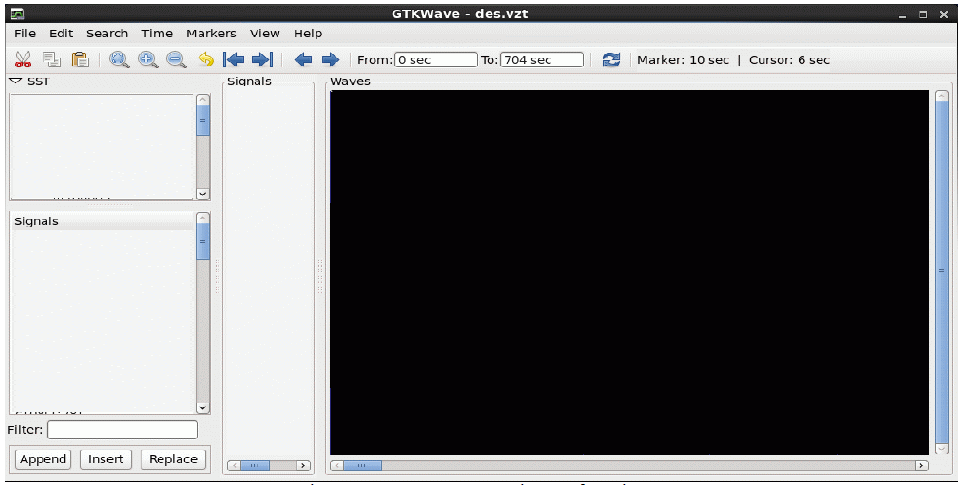
\includegraphics[scale=0.6]{1.png}
	\caption{Primera vista gráfica de GTKWave}
	\label{fig1}
\end{figure}
\noindent
A continuación se cargan las señales que se necesitan (Recuadros de la izquierda), se seleccionan y se arrastran hasta el panel vacío. Dado que todas las señales no están activadas es necesario hacerlo, para ello es necesario editar el archivo $system.v$, situado en \textit{SIE/SoftCore/lm32/logic/sack}.
\lstset{numbers=left, numberstyle=\tiny, stepnumber=1, numbersep=1pt}
\begin{lstlisting}[firstnumber=7, caption=Codigo inicial, label=code1]
 module system
 #(
 //	parameter   bootram_file     = "../firmware/cain_loader/image.ram",	
 //	parameter   bootram_file     = "../firmware/boot0-serial/image.ram",
	parameter   clk_freq         = 50000000,
	parameter   uart_baud_rate   = 57600
\end{lstlisting}
\noindent
El codigo \ref{code1} se debe descomentar en la linea $9$ o $10$, depende en que carpeta se valla a trabajar para realizar la compilación correcta, debe quedar como el cogido \ref{code2}
\begin{lstlisting}[firstnumber=7, caption=Código para trabajar en boot0-serial, label=code2]
 module system
 #(
 //	parameter   bootram_file     = "../firmware/cain_loader/image.ram",	
	parameter   bootram_file     = "../firmware/boot0-serial/image.ram",
	parameter   clk_freq         = 50000000,
	parameter   uart_baud_rate   = 57600
\end{lstlisting}
\noindent
Si se ha hecho este procedimiento bien al compilar en al carpeta \textit{sack/}, con el comando \textit{make view} saldrán todas las señales que tiene el procesador para eso se debe fijar en la parte izquierda de la pantalla, en estos dos recuadros se encuentran dichas señales, escogen las que necesitan.\\
Al realizar el paso mencionado anteriormente  y al seleccionar las señales el simulador se observara como en la figura \ref{fig2}.
\begin{figure}[H]
	\centering
		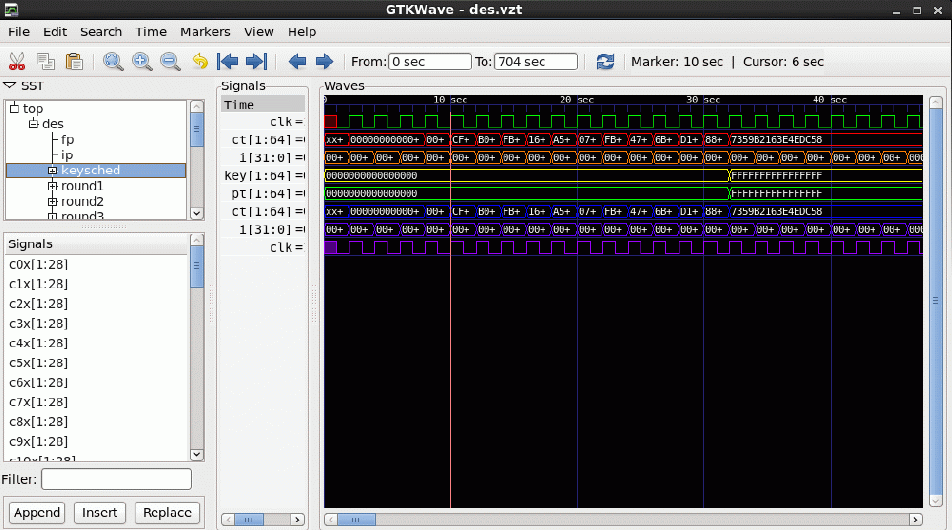
\includegraphics[scale=0.6]{2.png}
	\caption{Señales cargadas al GTKWave}
	\label{fig2}
\end{figure}

\subsection{Cargar señales seleccionadas de la simulación anterior}
\noindent
Como se han podido dar cuenta al simular con GTKWave siempre se tienen que cargar las señales que se van a visualizar, si se esta trabajando en un proyecto o haciendo simulaciones sobre un programa en especifico es muy complicado y realmente molesto tener que cargar cada vez que se quiera simular todas las señales que se quieren visualizar. Por tal motivo a continuación se presenta una forma más fácil de cargar estas señales automáticamente siempre y cuando sean las mismas para cada simulación.
\begin{enumerate}
 \item Se cargan todas las señales que se quieren ver (Figura \ref{fig3a}).
 \item File – Write Save File As (Figura \ref{fig3b}).
 \item Se dirige a la carpeta \textit{SIE/SoftCore/lm32/sie} busca el archivo $system\_tb.vcd.save.sav$, da click en salvar y en la alerta que aparece le dan replace (Figura \ref{fig3c}).
 \item Ahora nuevamente a la consola y se ejecuta el comando \textit{make view} y cuando se habrá GTKWave aparecerá la simulación con todas las señales que se han estado usando.
\end{enumerate}
\begin{figure}[H]
    \centering
        \subfigure[Cargar las señales]{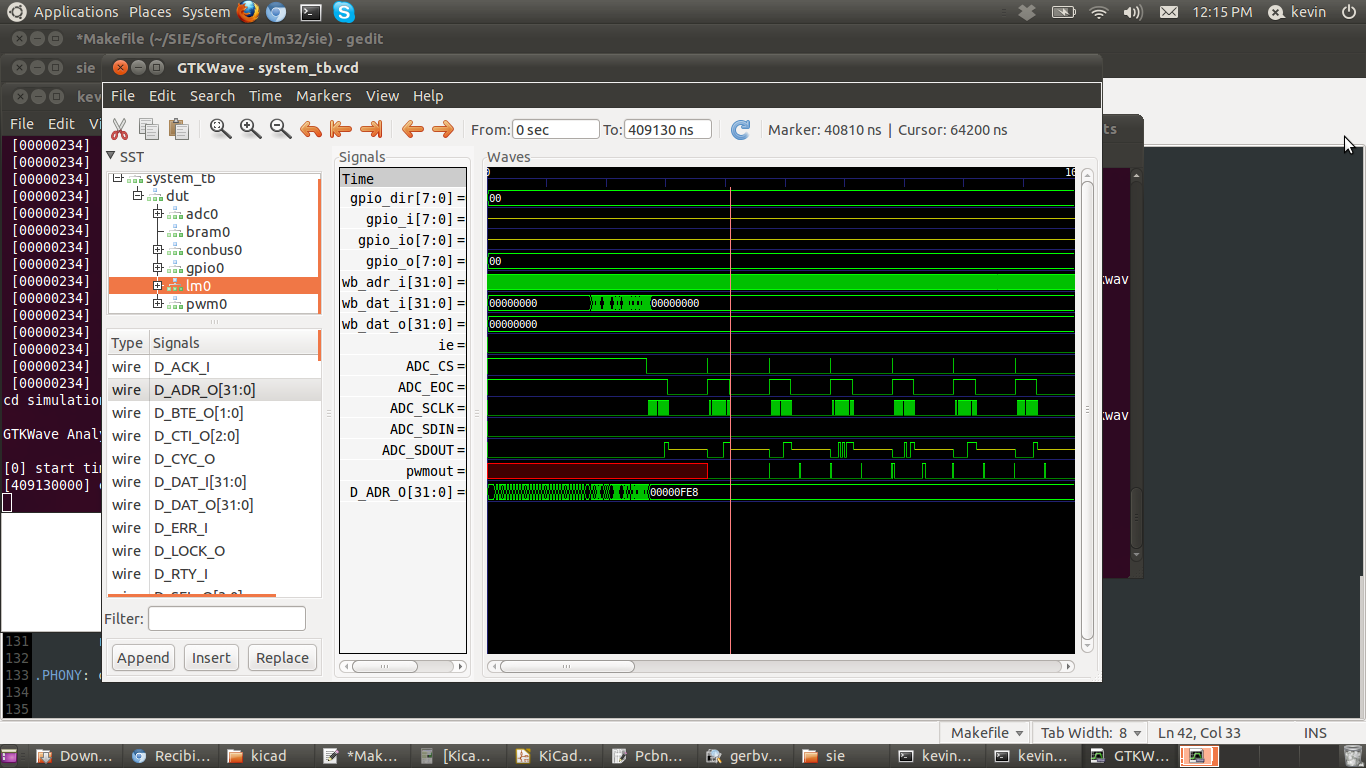
\includegraphics[scale=0.26]{image1.png}\label{fig3a}}
        \subfigure[Buscar la carpeta \textit{sack/}]{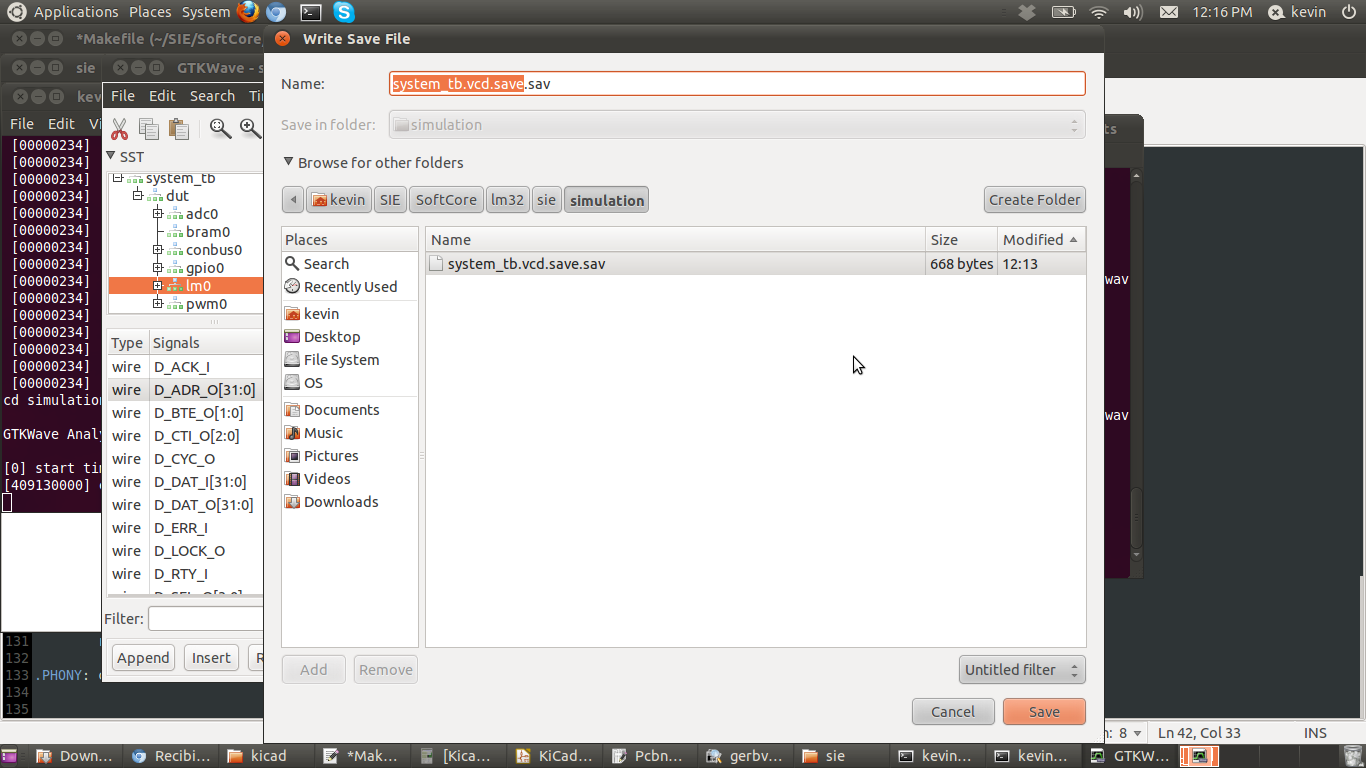
\includegraphics[scale=0.26]{image2.png}\label{fig3b}}
        \subfigure[Sobre escribir el archivo de la carpeta]{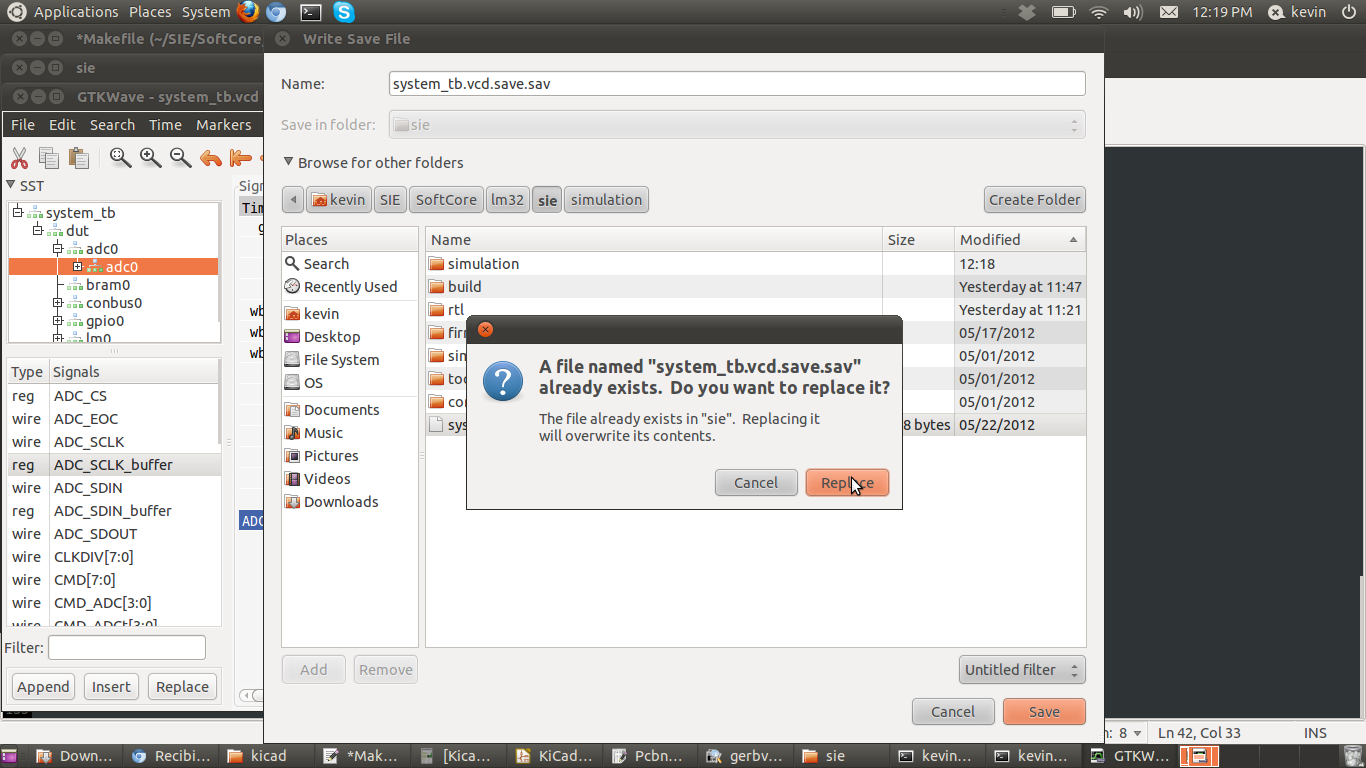
\includegraphics[scale=0.26]{image3.png}\label{fig3c}}
\caption{Pasos a seguir para cargar las señales}
\label{fig3}
\end{figure}

\section{Comó funciona GTKWave}
\begin{enumerate}
 \item GTKWave espera un archivo. Vcd que se genera a partir de una ejecución de simulación como entrada. Aquí, vamos a suponer que la entrada se fibonacci.vcd que se genera mediante la compilación y simulación ``fibonacci.v''.
 \item Invocar GTKWave: \textit{bash-2.05a \$ GTKWave filename.vcd} un seguimiento de la muestra es la siguiente. La ayuda en línea está disponible para todas las funciones de menú en GTKWave.\\
Con el fin de acceder a la ayuda en línea, seleccione Help-Wave Ayuda en el menú y luego seleccionar cualquier opción de menú para ver la descripción de la opción de menú.
 \item Seleccione la opción Search $\rightarrow$ Search Tree de la señal. Esto abrirá una nueva ventana. Se ofrece como un medio fácil de añadir las huellas de la pantalla en forma de árbol de un texto basado en la moda. El objetivo principal es añadir las señales a la pantalla para la visualización.\\
Árbol de la señal de búsqueda proporciona un medio fácil de añadir las huellas de la pantalla. Varias funciones se proporcionan en el árbol de búsqueda de señales que permiten la búsqueda de una jerarquía de árbol. Ahora selecciona las señales desde el árbol de búsqueda de la señal y haga clic en el botón Añadir. Las señales correspondientes se añaden a la pantalla. Del mismo modo, se puede insertar o cambiar las señales de la pantalla usando la inserción o reemplazar la ficha.
 \item Ahora estamos listos para ver y analizar las formas de onda de nuestro diseño. La ventana de la pantalla se divide en partes, a saber las señales de la ventana y ventana de ondas. Podemos observar los valores de las señales en cualquier instante particular del tiempo haciendo clic con el ratón en ese punto en la ventana de la señal.\\
Lo que sigue a continuación es la lista y descripción de los elementos de menú de uso común
    \begin{enumerate}
     \item Para imprimir el resultado en un archivo use la opción File $\rightarrow$ Print to File, que le preguntará por el nombre de PostScript encapsulado para generar las actuales pantallas de la ventana principal de su contenido.
     \item Para establecer el formato de visualización de datos utiliza la opción Edit $\rightarrow$ Data format. Se mostrará un conjunto de opciones como decimal, binario, hexadecimal, etc opciones pasará por todos los rastros de relieve y garantizar que el vector con esta clasificación se muestran con valores hexadecimales. Del mismo modo podemos elegir otras opciones.
     \item Podemos buscar formas de onda usando la opción Search $\rightarrow$ pattern Search. Patrón de búsqueda sólo funciona cuando al menos uno de seguimiento se puso de relieve (haciendo clic en la señal). La solicitud se parece que se enumeran todos los restos seleccionados y permite diferentes criterios que se especifican para cada trazo.\\
La búsqueda puede seguir adelante hacia atrás a partir de la marca primaria no identificada.
    \end{enumerate}
\end{enumerate}

\subsection{¿Como encontrar el dato que se requiere en la simulación?}
\noindent
Dado que GTKWave muestra las señales cuadradas no se puede interpretar bien el dato, además aparece en formato Hexadecimal.\\
Para encontrar los datos es necesario seguir los siguientes pasos:
\begin{enumerate}
 \item Al tener las señales cargadas en GTkwave (Figuras \ref{fig2} o \ref{fig3a}) en el segundo cuadro \textit{Signals-Time}
 \item Se seleccionan las señales que se desean cambiar de formato, como se encuentra en Hexadecimal se quiere cambiar decimal, entonces se ingresa a Edit$\rightarrow$Data Format$\rightarrow$Decimal, o también se oprime ALT+D.
 \item Luego se ingresa a Search$\rightarrow$Pattern Search 1, aparecera la figura \ref{fig4}
\begin{figure}[H]
	\centering
		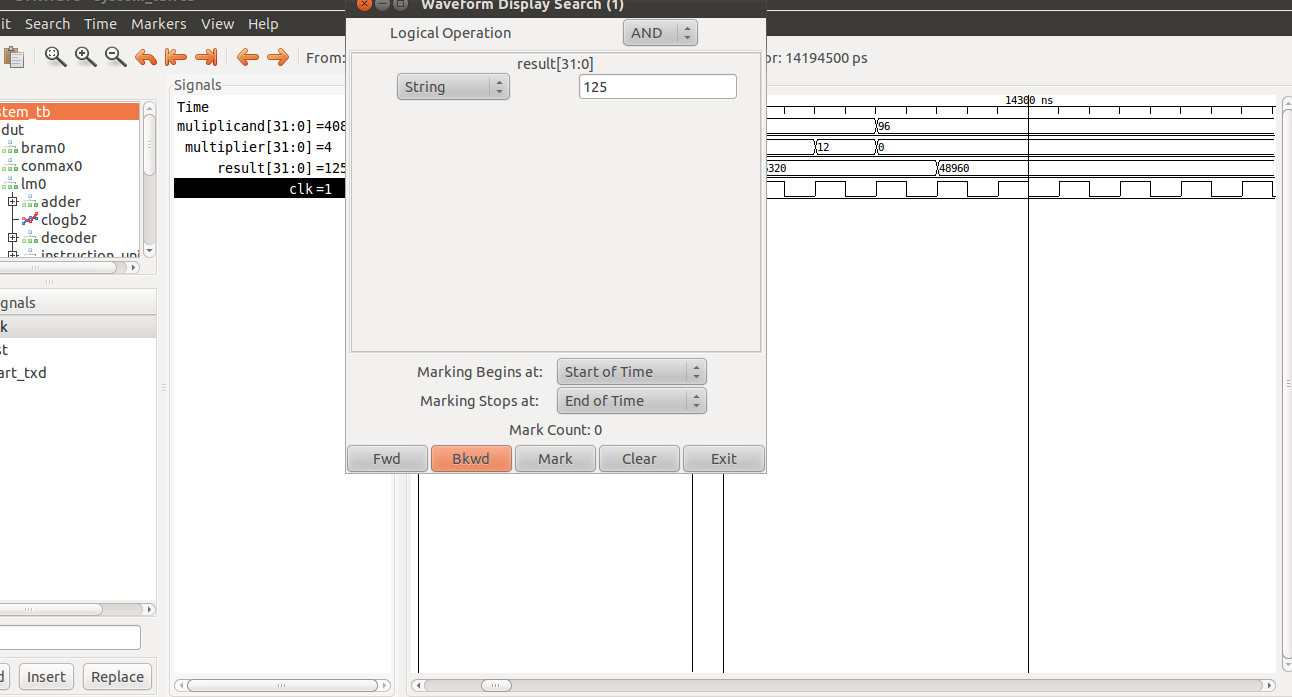
\includegraphics[scale=0.4]{4.png}
	\caption{Opción de búsqueda GTKWave}
	\label{fig4}
\end{figure}
\noindent
y se dejara como esta en dicha figura.
 \item Luego se escribe el dato que se desea buscar y se le da \textit{Bkwd}, así encontrara el dato que desea buscar.
\end{enumerate}

\subsection{¿Como se puede guardar la simulación en un archivo de imagen o PDF?}
\noindent
Primero se debe obtener las señales como las Figuras \ref{fig2} o \ref{fig3a}, se ingrese en File$\rightarrow$Print to file, y lo guarda en el formato que lo requiera, u oprimiendo CTRL+P.

\section{Ejemplos}
\subsection{Ejemplo 1}
\noindent
Este ejemplo tiene el siguiente código en C
\lstset{numbers=left, numberstyle=\tiny, stepnumber=1, numbersep=1pt}
\begin{lstlisting}[firstnumber=1, caption=Ejemplo 1 - Multiplicación, label=code2]
 #include <stdio.h>
 int main(){
	volatile unsigned int multiplicador, multiplicando,producto;
	multiplicador=25;
	multiplicando=5;
	producto=0;*
	producto = multiplicador * multiplicando;
	return 0;
 }
\end{lstlisting}
\noindent
Al realizar el procedimiento anterior se obtuvo como resultado
\begin{figure}[H]
	\centering
		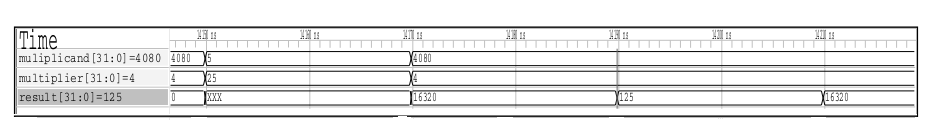
\includegraphics[scale=0.55]{example1.png}
	\caption{Ejemplo 1}
	\label{fig5}
\end{figure}

\subsection{Ejemplo 2}
\noindent
Este ejemplo tiene el siguiente código en C
\begin{lstlisting}[firstnumber=1, caption=Ejemplo 2 - Sumas sucesivas, label=code2]
 # include"stdio.h"
 int main(){
	volatile unsigned int multiplicador,multiplicando,producto,contador;
	multiplicador=7;
	multiplicando=25;
	producto=0;
	contador=0;
	for (contador=0; contador<multiplicador; contador++){
        	producto=producto+multiplicando;                                        
	};
	return 0;
 }
\end{lstlisting}
\noindent
Al realizar el procedimiento anterior se obtuvo como resultado
\begin{figure}[H]
	\centering
		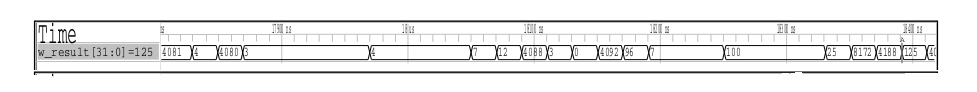
\includegraphics[scale=0.55]{example2.png}
	\caption{Ejemplo 2}
	\label{fig6}
\end{figure}

\bibliographystyle{ieeetran}
\begin{thebibliography}{99}
\bibitem{page1} \url{http://gtkwave.sourceforge.net/gtkwave.pdf}
\end{thebibliography}
\end{document}